% =====================================================================
% Pacotes adicionais e adaptação do template para português.
% A pasta configs/ não foi alterada: os comandos com textos fixos em
% inglês são redefinidos aqui, depois do carregamento da classe.
% =====================================================================

\usepackage{booktabs}
\usepackage{tabularx}
\usepackage{longtable}
\usepackage{array}
\usepackage{multirow}
\usepackage{float}
\usepackage[font=small,labelfont=bf,justification=centering]{caption}
\usepackage{enumitem}
\usepackage{listings}
\usepackage{ragged2e}
\usepackage{rotating}
\usepackage{xurl}

% Quebra de linha manual em títulos de capítulo: vira espaço no sumário
\newcommand{\quebraimpl}{}
\DeclareRobustCommand{\quebra}{\quebraimpl}

\hypersetup{hidelinks}
\urlstyle{same}

\newcolumntype{L}[1]{>{\RaggedRight\arraybackslash}p{#1}}
\newcolumntype{Y}{>{\RaggedRight\arraybackslash}X}
\setlist{itemsep=2pt,topsep=4pt}

% Fonte das figuras e tabelas, conforme a ABNT
\newcommand{\fonte}[1]{\par\vspace{2pt}{\centering\small Fonte: #1\par}}

% Listagens de código
\lstdefinestyle{codigo}{
  basicstyle=\ttfamily\footnotesize,
  breaklines=true,
  frame=single,
  rulecolor=\color{gray!60},
  backgroundcolor=\color{gray!6},
  columns=fullflexible,
  keepspaces=true,
  showstringspaces=false,
  inputencoding=utf8,
  extendedchars=true,
  literate={á}{{\'a}}1 {é}{{\'e}}1 {í}{{\'i}}1 {ó}{{\'o}}1 {ú}{{\'u}}1
           {ã}{{\~a}}1 {õ}{{\~o}}1 {ç}{{\c{c}}}1 {ê}{{\^e}}1 {â}{{\^a}}1
           {ô}{{\^o}}1 {Á}{{\'A}}1 {É}{{\'E}}1 {Ç}{{\c{C}}}1
}
\lstset{style=codigo}
\renewcommand{\lstlistingname}{Código}

% ---------------------------------------------------------------------
% Idioma principal: português
% ---------------------------------------------------------------------
\addto\captionsportuguese{%
  \renewcommand{\refname}{\color{titulos}\bfseries\MakeUppercase{Referências}}%
  \renewcommand{\figurename}{Figura}%
  \renewcommand{\tablename}{Tabela}%
}
\AtBeginDocument{\selectlanguage{portuguese}}

% ---------------------------------------------------------------------
% Folha de rosto
% ---------------------------------------------------------------------
\renewcommand{\folharosto}{
    \clearpage
    \thispagestyle{pretext}
    \begin{flushleft}
        {\Large\bfseries\color{fundo_idp}\MakeUppercase\autornome}

        \vspace*{3cm}
        {\Large\color{fundo_idp}\MakeUppercase\titulonome}

        \vspace*{3cm}

        \noindent{Trabalho de Conclusão de Curso apresentado como requisito
        parcial para a obtenção do título de Bacharel em \nomecurso{} pelo
        Instituto Brasileiro de Ensino, Desenvolvimento e Pesquisa (IDP).}

        \vspace*{3cm}

        {\bfseries\color{fundo_idp}
        \iforientadora Orientadora
        \else Orientador
        \fi}\\
        {\nomeorientador}

        \vspace*{3cm}
        {Brasília - DF, \anonome}
    \end{flushleft}
}

% ---------------------------------------------------------------------
% Folha de aprovação
% ---------------------------------------------------------------------
\renewcommand{\folhaaprovacao}{
    \clearpage
    \thispagestyle{pretext}
   \begin{flushleft}
        {\Large\bfseries\color{fundo_idp}\MakeUppercase\autornome}

        \vspace*{3cm}
        {\Large\color{fundo_idp}\MakeUppercase\titulonome}

    \end{flushleft}
        \vspace*{2cm}

        \noindent{Trabalho de Conclusão de Curso apresentado como requisito
        parcial para a obtenção do título de Bacharel em \nomecurso{} pelo
        Instituto Brasileiro de Ensino, Desenvolvimento e Pesquisa (IDP).}

    \begin{flushleft}

        \vspace*{2cm}
        {Aprovado em \dataaprovacaoVal}

        \vspace*{1cm}
        {\bfseries\color{fundo_idp}Banca Examinadora}

        {
        \vspace*{2cm}
        \vspace{1em}
        {\nomeorientador\ (\iforientadora Orientadora\else Orientador\fi) - \instorientador}

        \vspace*{2cm}
        \vspace{1em}
        {\nomemembrobancai\ (\funcaomembrobancai) - \instbancai}

        \vspace*{2cm}
        \vspace{1em}
        {\nomemembrobancaii\ (\funcaomembrobancaii) - \instbancaii}
        }
    \end{flushleft}
}

% ---------------------------------------------------------------------
% Elementos pré-textuais opcionais
% ---------------------------------------------------------------------
\renewcommand{\agradecimentos}{
    \clearpage
     \begin{flushleft}
    {\Large\bfseries\color{fundo_idp}\MakeUppercase{Agradecimentos}}
    \end{flushleft}
    \vspace{1em}
    \lipsum[1]
}

\renewcommand{\dedicatoria}{
    \clearpage
     \begin{flushleft}
    {\Large\bfseries\color{fundo_idp}\MakeUppercase{Dedicatória}}
    \end{flushleft}
    \vspace{1em}
    \lipsum[1]
}

% ---------------------------------------------------------------------
% Capa das referências
% ---------------------------------------------------------------------
\renewcommand{\capareferencias}{
    \clearpage
    \thispagestyle{empty}
    \AddToShipoutPicture*{
        \put(-3,0){
            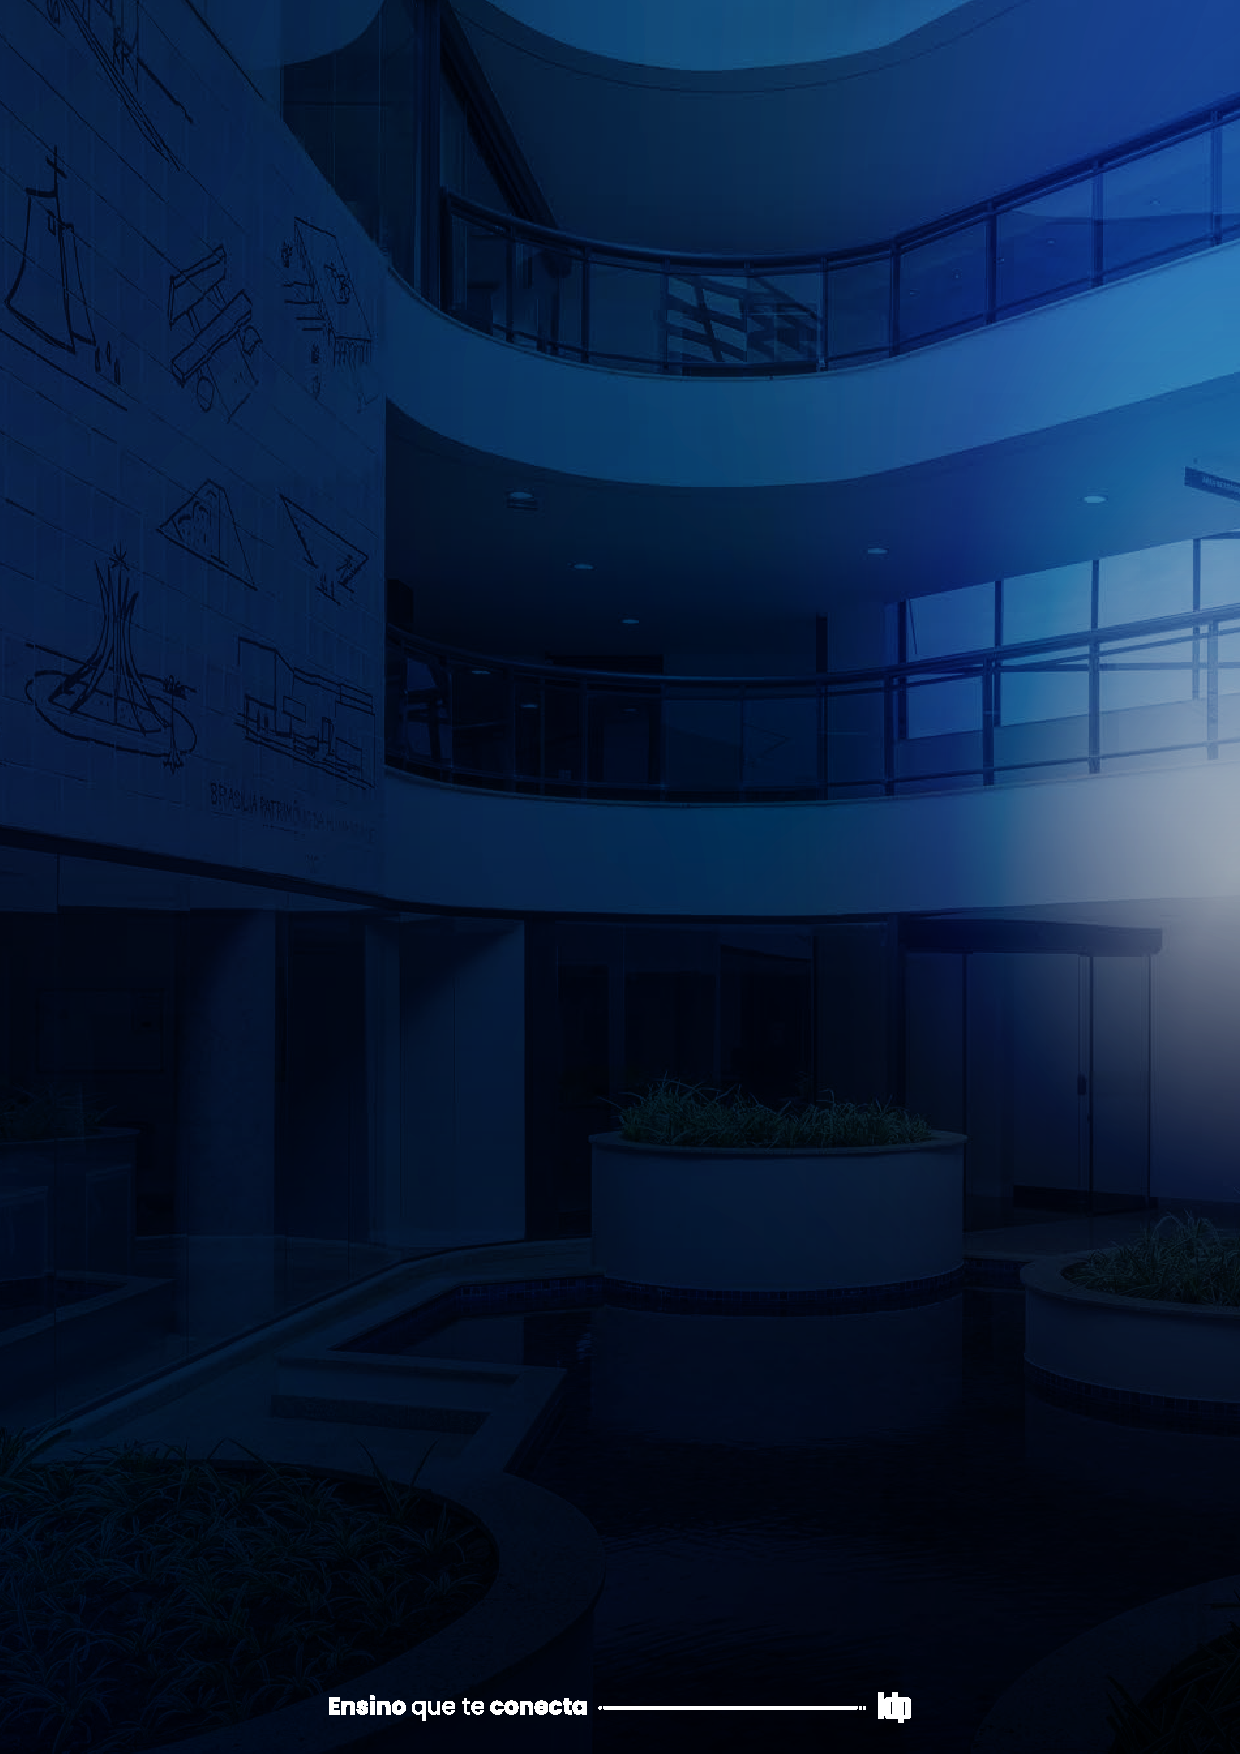
\includegraphics[width=\paperwidth,height=\paperheight]{configs/figuras/capa_secoes.pdf}
        }
    }
     \color{white}

    \vspace*{\fill}
    \begin{center}
    {\fontsize{60}{0}\bfseries\MakeUppercase{Referências}}
    \end{center}
    \vspace*{\fill}

    \refstepcounter{secnum}
    \phantomsection
    \addcontentsline{toc}{section}{Referências}

    \color{black}

    \null
    \clearpage
}

% ---------------------------------------------------------------------
% Apêndices
% ---------------------------------------------------------------------
\makeatletter
\renewcommand{\apendice}[3][]{%
        \clearpage
        \stepcounter{apendicecount}%
        \ifnum\value{apendicecount}=1
                \capaapendice{Apêndices}
        \fi
        \phantomsection
        \addcontentsline{toc}{section}{Apêndice \MakeUppercase{\alph{apendicecount}} - #2}
        \begin{center}
                {\color{fundo_idp}\Large{Apêndice \MakeUppercase{\alph{apendicecount}} - #2}}
        \end{center}
        \ifx&#1&%
                \edef\tempaplabel{ap:\alph{apendicecount}}%
                \labelapendice{\tempaplabel}%
        \else
                \labelapendice{#1}%
        \fi
        \input{#3}
}
\makeatother
